\documentclass{article}

% if you need to pass options to natbib, use, e.g.:
%     \PassOptionsToPackage{numbers, compress}{natbib}
% before loading neurips_2021

% ready for submission
\usepackage[preprint]{neurips_2021}

% to compile a preprint version, e.g., for submission to arXiv, add add the
% [preprint] option:
%     \usepackage[preprint]{neurips_2021}

% to compile a camera-ready version, add the [final] option, e.g.:
%     \usepackage[final]{neurips_2021}

% to avoid loading the natbib package, add option nonatbib:
% \usepackage[nonatbib]{neurips_2021}

\usepackage[utf8]{inputenc} % allow utf-8 input
\usepackage[T1]{fontenc}    % use 8-bit T1 fonts
\usepackage[colorlinks = true, 
		    linkcolor = blue,
		    urlcolor  = blue,
            citecolor = blue,
            anchorcolor = blue]{hyperref}       
% hyperlinks
\usepackage{url}            % simple URL typesetting
\usepackage{booktabs}       % professional-quality tables
\usepackage{amsfonts}       % blackboard math symbols
\usepackage{nicefrac}       % compact symbols for 1/2, etc.
\usepackage{microtype}      % microtypography
\usepackage{xcolor}         % colors
\usepackage{natbib}
\usepackage[pdftex]{graphicx}
\usepackage{siunitx} % Required for alignment
\sisetup{
  round-mode          = places, % Rounds numbers
  round-precision     = 2, % to 2 places
}
	
\bibliographystyle{unsrtnat}


\title{Spotify metadata: Pop music is really less diverse}

% The \author macro works with any number of authors. There are two commands
% used to separate the names and addresses of multiple authors: \And and \AND.
%
% Using \And between authors leaves it to LaTeX to determine where to break the
% lines. Using \AND forces a line break at that point. So, if LaTeX puts 3 of 4
% authors names on the first line, and the last on the second line, try using
% \AND instead of \And before the third author name.

\author{%
  Dominik Glandorf\\
  Matrikelnummer 6007407\\
  \texttt{dominik.glandorf@student.uni-tuebingen.de} \\
  \And
  Felix Gross\\
  Matrikelnummer 6001480\\
  \texttt{fel.gross@student.uni-tuebingen.de} \\
}

\begin{document}

\maketitle

\begin{abstract}
% What did we do?
In this work we investigated if popular music is less diverse in terms of its variability.
% Why did we to it? What did we expect?
To assess the cliché of contemporary pop music "being all the same",
% How did we do it?
metadata of 28,195 tracks on Spotify was collected, notably their popularity and audio features. To compare variability within popular versus non-pop songs, a Principal Component Analysis and F-tests were conducted.
% What did we find out?
A 2D-plot visually showed a difference between the groups. An analysis of variance confirmed that the diversity is indeed less in pop music, confirming our initial hypothesis.
% What now?
Conclusively, we discussed our findings' generalizability, challenged by a potential sampling bias. 
%and imbalanced data.
\end{abstract}

\section{Introduction}
%Why are we interested in music?
Music is one of the oldest and most valued forms of communication and therefore of particular interest. Yet, its underlying structure has been eluded systematic analysis until recently.
% What can we contribute?
Accelerated computing and freely accessible databases allow now for systematic inquiry of numerous features across thousands of songs. Thus, it is only now possible to hold common clichés about music proof to the real world data.
% What is our research question?
One of these clichés is, that pop music is all the same and less diverse then non-popular music \citep{serra2012measuring}. Thus, our hypothesis is, that the variability of pop music is smaller than the one observed in non-popular music.

% What does music and popularity mean to us?
% TODO: add source for usage statistics and number of tracks
Since Spotify is the world's most used music streaming platform and offers one of the largest corpora of music \citep{quarterlyReport}, it promises it to be representative for global listening preferences. For this reason, we rely on this single platform to define what is considered as music, as well as what is considered as popular music. Spotify's massive amount of listening data allows to assess which songs are popular and its meta knowledge eases the examination of music out of a quantitative perspective.
% What is variability?
We define variability (and synonymously diversity) in the statistical sense of variance, i.e. the average squared distance from the mean. This variability between songs, is expected to be reflected in objective measures like tempo, or more subjective ones like "danceability".  The latter, ambiguous properties  are calculated by Spotify utilising usage statistics and audio analysis.

\section{Method}

\subsection{Sample}
% Where did we get the data exactly from?
% How did exactly did we request our data?
Our sample was obtained from the Spotify audio endpoint in the following way: For each possible single Latin letter and two letter combination, the 50 first search results including their popularity score were stored. After eliminating duplicates in the result lists, the total sample encompassed 28,195 songs. To the list of songs were then added the metadata of the Spotify Web API \citep{spotifyDocu}.
% What are the columns/groups of our dataset?  
The obtained features are explained in Table \ref{tab:features}. We defined a song being a pop song, if is popularity value is equal or above 90. 70 songs fulfilled this criterion, and were then assigned to the pop song group. The remainder of 28,125 was assigned to the non-pop song group. 

%use [!t] to move figures, figure* is required
\begin{figure*}[!b]
  \centering
  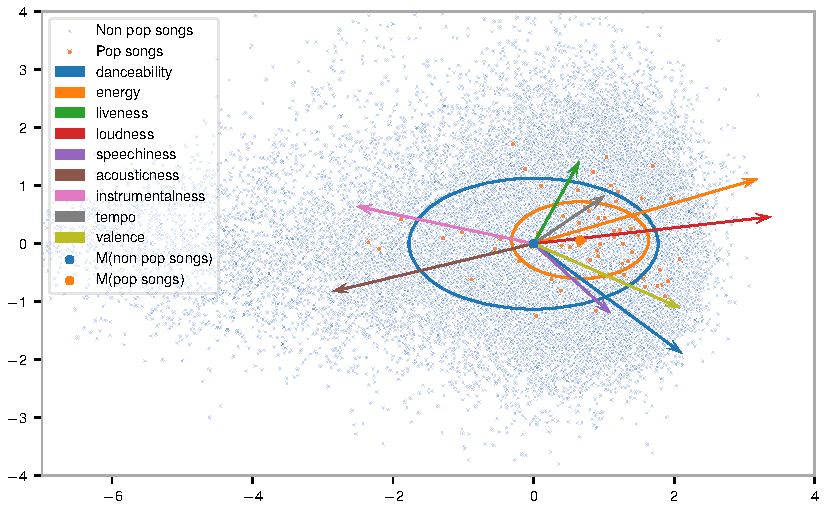
\includegraphics[]{../fig/001_pca.pdf}
  \vspace*{-8mm}  
  \caption{The projected sample on the first two principal components}
  \label{fig:pca}
\end{figure*}

\begin{table}[t]
  \centering
  \begin{tabular}{ll}
    \toprule
    Feature     & Description\\
    \midrule
	danceability        	& Describes how suitable a track is for dancing  \\
	energy              	&  Represents a perceptual measure of intensity and activity from 0.0 to 1.0\\
	liveness            	&  Detects the presence of an audience in the recording\\
	loudness            	&  The overall loudness of a track in decibels (dB)\\
	speechiness         	&  Detects the presence of spoken words in a track\\
	acousticness        	& A confidence measure from 0.0 to 1.0 of whether the track is acoustic	\\
	instrumentalness    	&	Predicts whether a track contains no vocals. \\
	tempo               	&  The overall estimated tempo of a track in beats per minute (BPM)\\
	valence             	& Describes the musical positiveness conveyed by a track from 0.0 to 1.0\\
	\midrule
	popularity           &  A value from 0 to 100 is assigned to each song, 100 being the most popular\\
    \bottomrule
  \end{tabular}
  \vspace*{2mm}
  \caption{The inspected features}
  \label{tab:features}
\end{table}


\subsection{Analysis}
% How did we ensure our data are appropriate?
To ensure data quality, we first graphically and numerically checked the distributions of our audio features and the popularity in the sample.

% How did we visually approached our hypothesis?
As stated above, we were interested in the variability of pop songs compared to the remainder. Hence, we first employed an exploratory and visual approach before running statistical tests. In order to search for an underlying structure in the audio features and to be able to get a first impression of the data as a whole, we decided to do a dimensionality reduction via Principal Component Analysis (PCA). We did not use a stochastic neighbour embedding such as t-SNE since we only have nine dimensions and assumed a global structure that might not be preserved by those methods. To be able to plot the principal components we chose the two components that explained the most variance. Since the PCA is agnostic to the grouping we indicated the class labels in the visualization, in hope to see a structure. If there are common components in the feature space it is probable that we already see a difference in variance in the visualized data.

% How did we statistically approached our hypothesis?
Independently of the results of the data exploration, we planned to conduct a two sample variance comparison on each audio feature \citep{snedecor1989}. Since our hypothesis, was not comprised out of mean differences in the two groups but rather on variance differences, the method of choice was a classical F-test for independent samples. To account for our multiple tests, we corrected our critical f-value using the Bonferroni method. To further assess robustness of our point estimation, we ran a bootstrap sampling from both groups and calculated the variance quotient, i.e. the F-statistic for each of the 10,000 resampled pairs of groups. According to \cite{kruschke2014}.
we calculated the 95\% highest density interval (HDI) that contains the 95\%  most often encountered variance ratios obtained in the bootstrap procedure. This allows for corrobating the F-test results, because we get an interval, in which we expect our statistics to lie with a high confidence after re sampling the data.

\section{Results}

% TODO: create this from the right file
% only one legend, and maybe horizontal boxplots to variance
\begin{figure}
  \centering
  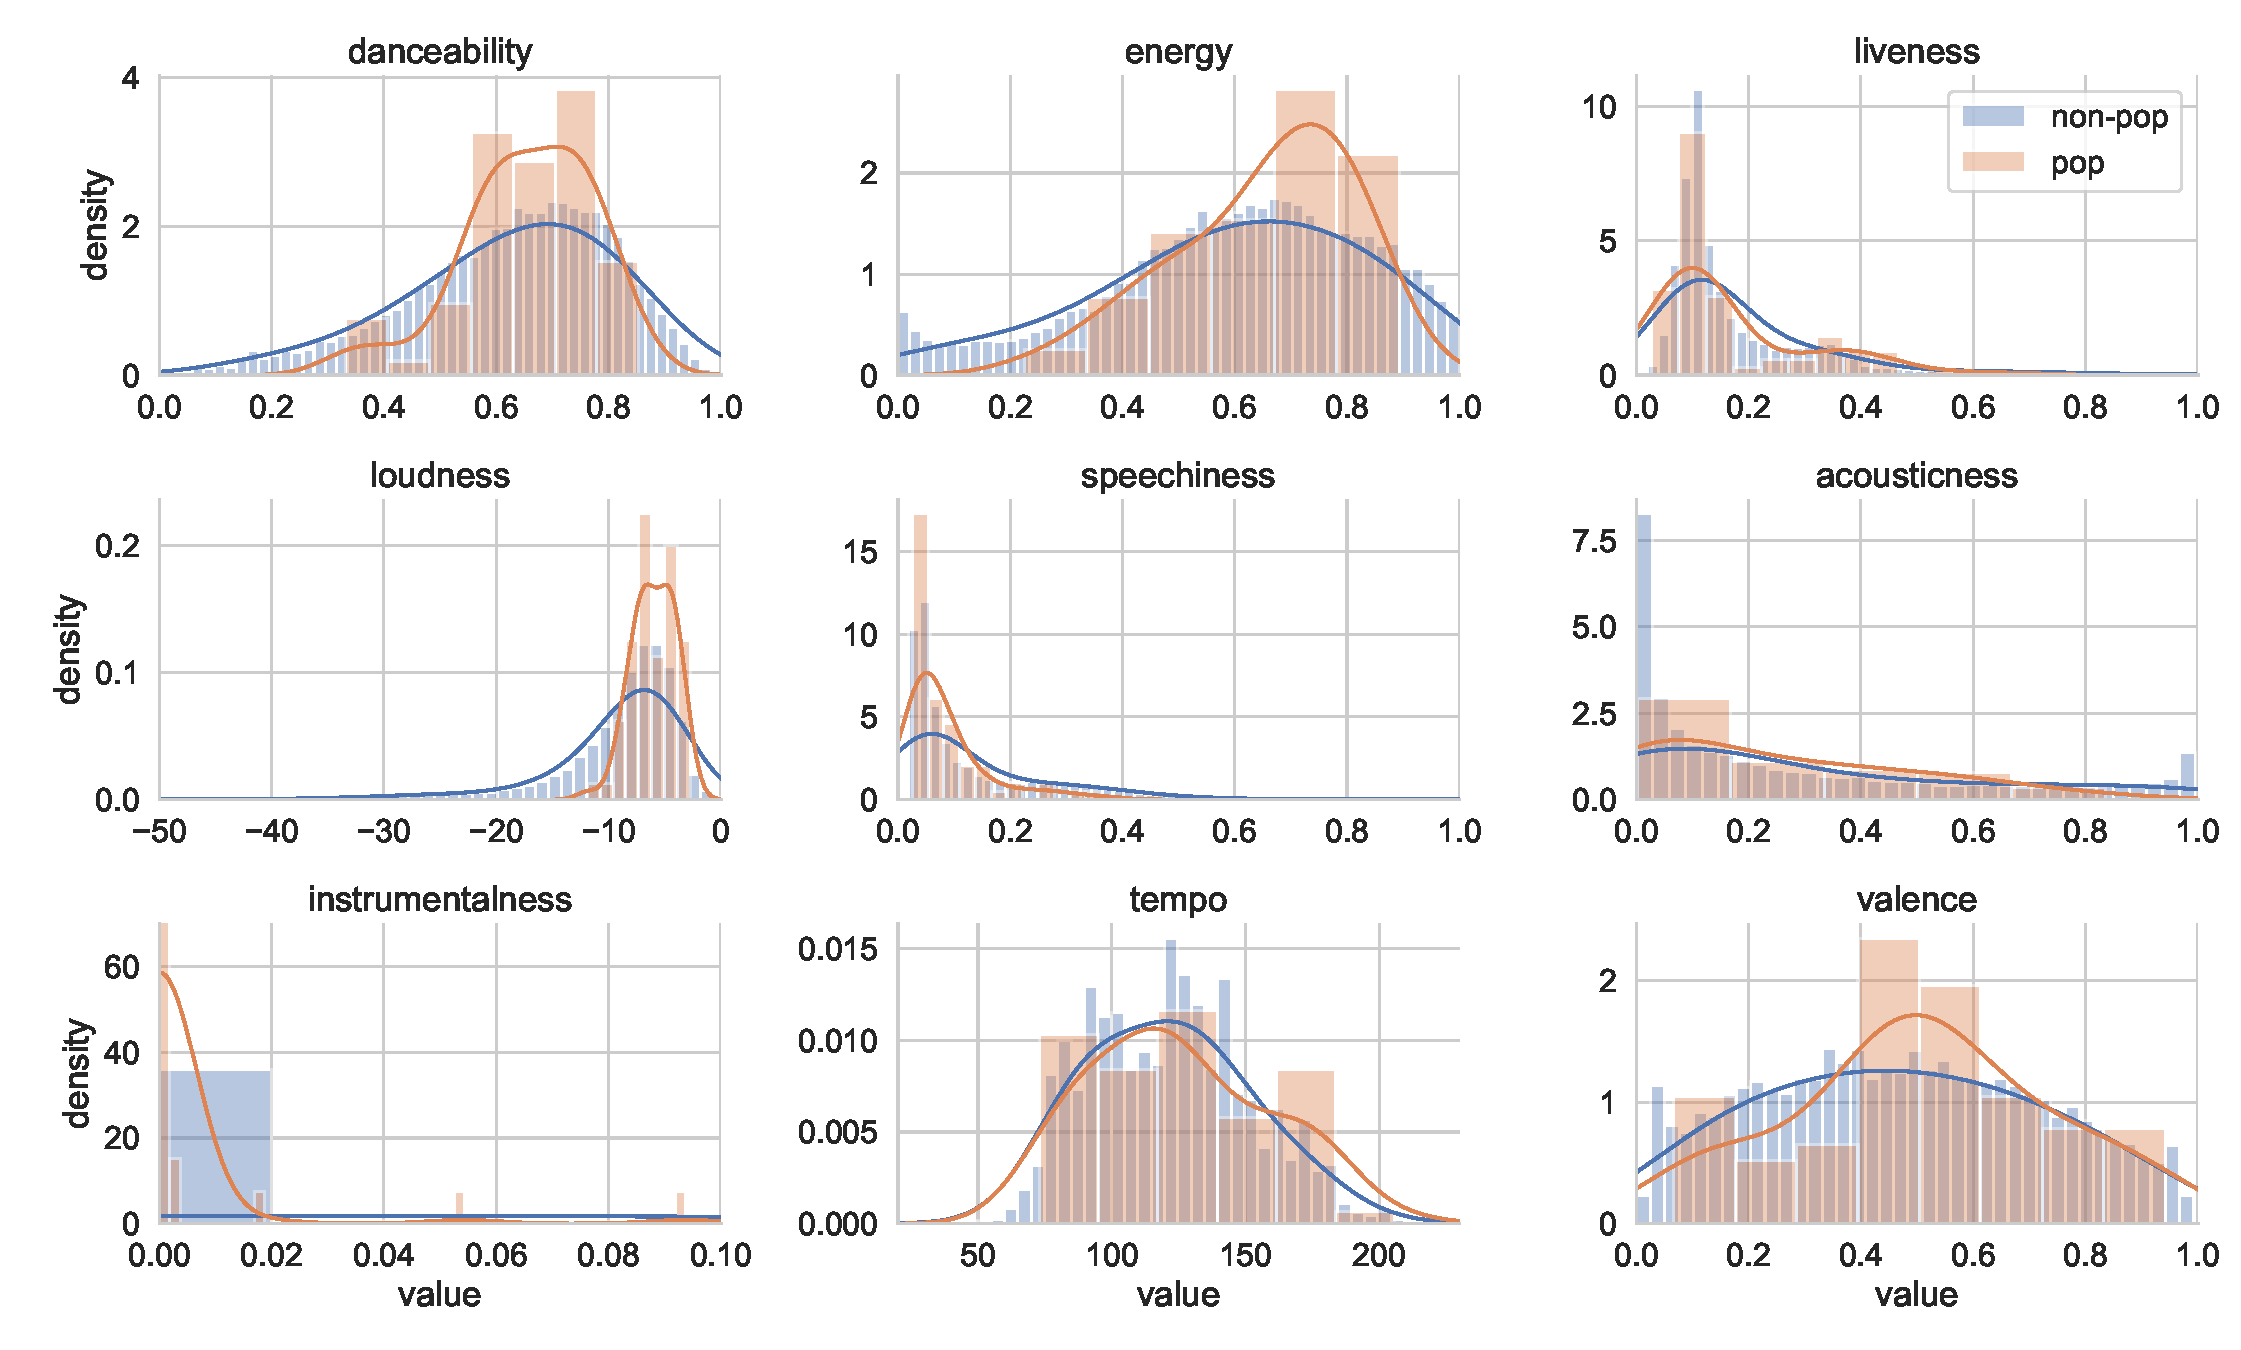
\includegraphics[width=1\linewidth]{../fig/002_variances.pdf}
  \vspace*{-8mm}
  \caption{Variances of all inspected features}
\end{figure}

%We will first evaluate our graphical analysis, then the statistical procedures to find out if there are different variabilities in the two groups. 
In Figure \ref{fig:pca} a 2D-visualization of the projected data points is shown. The popular songs clearly spread over an area contained in the bandwidth of the remaining songs. The standard variance within the first two principal components (PC) is visualized via the ellipses around the group means. This underlines the visual impression of lower variance of the popular songs. The mean of them is positively shifted mainly on the first PC. To understand how the original features load onto the PCs their loadings are indicated in an arbitrary scale via the arrows originating from the data's origin. The first PC is mainly determined by loudness and energy (positive loading) as well as instrumentalness and acousticness (negative loading). This PC could be seen as the "pop" dimension since today's popular songs are generally known to be energetic and well-produced (which results in a higher loudness feature) and less instrumental or acoustic (since those are perceived as stripped versions of the original music). The second PC shows the same pattern of less variance in the pop songs, even though it is less prominent. It is mainly based on liveness, speechiness, valence, danceability and tempo. Due to the very small mean difference those features seem not to be different in popular songs, yet less variant. From the dimensionality reduction we can conclude that popular music seems to be actually less diverse in terms of its audio features and shows average differences.

\begin{table}[h!]
  
  \label{tab:var}
  \centering
  \begin{tabular}{lllc}
    \toprule
    Feature     & F-value & 95\% HDI\\
    \midrule
	danceability        	&  2.50** & [1.79; 3.38]\\
	energy              		&  2.26** & [1.79; 2.77]\\
	liveness            		&  1.23   & [0.85; 1.80]\\
	loudness            	&  9.27** & [7.53; 11.26]\\
	speechiness         	&  3.57** & [1.95; 6.92]\\
	acousticness        	&  1.80*  & [1.44; 2.20]\\
	instrumentalness    	&642.00** & -\\
	tempo               		&  0.83   & [0.69; 0.98]\\
	valence             	&  1.21   & [1.01; 1.43]\\
    \bottomrule
  \end{tabular}
  \vspace*{2mm}
  \caption{Variance test and bootstrapping results}
\end{table}

% TODO: caption explaining meaning of *

% F-test/Variance tests results
% which audio features are significant?
All features except for liveness, tempo and valence had a significantly lower variance among the pop songs. The highest ratio by far was observed in the instrumentalness feature indicating there is literally no variance within the pop songs.
% Bootstrap How robust were our point estimates of the test statistic
The bootstrap-based robustness estimation showed that the significant results are mostly robust to resampling and will result in at least 95\% in the same decision. One exception was the feature acousticness that was not significantly different in the whole HDI. Please note, for variances in instrumentalness the HDI could not be determined in a reasonable way due to its extreme ratio.

\section{Discussion}
% What is our main result?
Confirming the impression of the exploratory analysis, the variance of six of the evaluated nine features was significantly less in the pop-music group, if compared to the non-pop music group, hereby mostly supporting our hypothesis of pop music being all the same.
% Q: are we okay with the blackbox calculation of our features?
% A: We are not able to calculate them easily by ourselves so the spotify calculation is already a way more informative approach
Even though we could not gather any intelligence about how the feature values were measured on Spotify's side, we still opted to use them. An own synthesis of the raw data into interpretable features would have been beyond the scope of this report. 
% Q: is our sampling strategy adequate? what is popular music?
% A: We were interested in the most popular songs and they are very likely to be output first by the search function. Nonetheless we do not really know if the remainder is really representative for "unpopular songs". Maybe people refer to "less known but still listened by fans" music instead of the big tail of never listened songs on spotify? 
Our specific sampling strategy is very likely to have caught all of the songs, one would consider popular, nevertheless the remainder is sampled inadequately. For each letter combination we only took the fifty most popular songs, thereby omitting the really unpopular songs. Thus, our reference group is rather comprised out of "mediocre songs", then out of songs, which are not popular at all.   
% imbalanced data, justify why it is inherent in our analysis and why we think that our results are still not biased by this imbalance
The size of our pop song group reflects the length of Spotify's own Top Playlist and resembles the present radio repetoire. Furthermore, being popular often encompasses being sparse. So the tremendous sample size differences are inherent to our analysis. We accounted for it by using F-tests, which are quite robust against said differences. Furthermore, bootstrapping does not make any assumption about the distribution at all. 
% Q: Outlook and Future research ideas:% 
%the analysis should be redone with another pop threshold or using it categorically (for example 10 groups of popularity)
% A1: consider different markets/cultures, Spotify is heavily biased to Western music, replicate our analysis for each countries charts
% A2: Check over time, if there is a change or manifestation in variance ratios to have better robustness estimation than bootstrap.
Further studies might explore how a different interpretation of popularity would affect the analysis. For example our quite arbitrarily chosen threshold could be lowered, or popularity could be treated as categorically or even continuous variable. Albeit disproportionate growth in non western markets, these are still under-represented and a specific focus on the diversity of the music there, could be fruitful. Lastly a better way of testing our hypothesis was to elicit the data over time - which we had not. The resulting time series would allow for a better robustness, then the methods applied by us. Aiding in better understanding one of our oldest forms of communication - music.   


% TODO: Look at the output and repair capitalization and 

\bibliography{library.bib}

\end{document}
